\documentclass[11pt]{article}

% ==================================================================
%  Giai thich chi tiet hai kien truc: Baseline RoadTransformer (exp00)
%  va SE(2)-Equivariant SE2RoadNet (exp02 / exp02b, focal gamma = 1).
%  Bien dich bang XeLaTeX (tieng Viet + Times New Roman).
% ==================================================================

\usepackage{fontspec}
\setmainfont{Times New Roman}
\setsansfont{Segoe UI}
\setmonofont{Consolas}[Scale=0.82]

\usepackage[margin=2.3cm]{geometry}
\usepackage{amsmath,amssymb,amsthm,mathtools}
\usepackage{xcolor}
\usepackage{tikz}
\usetikzlibrary{positioning,arrows.meta,fit,backgrounds,calc,shapes.geometric}
\usepackage{listings}
\usepackage{booktabs}
\usepackage{array}
\usepackage{multirow}
\usepackage{enumitem}
\usepackage{caption}
\usepackage{float}
\usepackage[colorlinks=true,linkcolor=blue!55!black,urlcolor=teal,
            citecolor=blue!55!black]{hyperref}

% ----- mau -----
\definecolor{cA}{HTML}{1F6FEB}   % baseline blue
\definecolor{cB}{HTML}{2E7D32}   % SE2 green
\definecolor{cInk}{HTML}{1B1B1B}
\definecolor{cGrey}{HTML}{6A6A6A}
\definecolor{cBox}{HTML}{F4F6FA}
\definecolor{cBoxB}{HTML}{EAF3EC}
\definecolor{cKw}{HTML}{A626A4}
\definecolor{cStr}{HTML}{50A14F}
\definecolor{cCom}{HTML}{9A9A9A}
\definecolor{cNum}{HTML}{C18401}

% ----- listings (Python) -----
\lstdefinestyle{py}{
  language=Python,
  basicstyle=\ttfamily\footnotesize\color{cInk},
  keywordstyle=\color{cKw}\bfseries,
  stringstyle=\color{cStr},
  commentstyle=\color{cCom}\itshape,
  numberstyle=\tiny\color{cGrey},
  numbers=left, numbersep=7pt,
  showstringspaces=false,
  columns=fullflexible, keepspaces=true,
  breaklines=true, breakatwhitespace=true,
  frame=single, rulecolor=\color{cGrey!40},
  backgroundcolor=\color{cBox},
  xleftmargin=14pt, framexleftmargin=14pt,
  literate={->}{{$\to$}}1 {>=}{{$\ge$}}1 {<=}{{$\le$}}1
}
\lstset{style=py}

% JSON khong co san trong listings -> tu dinh nghia (dung '#' lam chu thich)
\lstdefinelanguage{json}{
  morestring=[b]",
  stringstyle=\color{cStr},
  comment=[l]{\#},
  commentstyle=\color{cCom}\itshape,
  literate=*{:}{{{\color{cKw}:}}}1 {\{}{{{\color{cGrey}\{}}}1 {\}}{{{\color{cGrey}\}}}}1
}

% ----- macros -----
\newcommand{\code}[1]{\textcolor{cInk}{\texttt{#1}}}
\newcommand{\fileA}{\code{exp00\_Basline.py}}
\newcommand{\fileB}{\code{exp02\_SE2Equivariant.py}}
\newcommand{\fileBb}{\code{exp02b\_gamma\_sweep.py}}
\newcommand{\R}{\mathbb{R}}
\newcommand{\SEtwo}{\mathrm{SE}(2)}
\newcommand{\SOtwo}{\mathrm{SO}(2)}
\newcommand{\kk}{\kappa}
\newcommand{\Rot}{\mathbf{R}}
\newcommand{\pt}{\mathbf{p}}
\newcommand{\tvec}{\mathbf{t}}

\theoremstyle{definition}
\newtheorem{prop}{Mệnh đề}
\newtheorem{defn}{Định nghĩa}

\newcommand{\chA}[1]{\textcolor{cA}{\textbf{#1}}}
\newcommand{\chB}[1]{\textcolor{cB}{\textbf{#1}}}

% tikz styles
\tikzset{
  blk/.style={draw=cGrey!70, rounded corners=2pt, fill=cBox,
              align=center, inner sep=5pt, font=\small},
  blkA/.style={blk, draw=cA!70, fill=cA!7},
  blkB/.style={blk, draw=cB!70, fill=cB!8},
  ar/.style={-{Stealth[length=6pt]}, cGrey!80, thick},
  tag/.style={font=\scriptsize\itshape, cGrey}
}

\title{\vspace{-1.2cm}\textbf{Hai kiến trúc cho SDC Test Prioritization}\\[4pt]
\large Baseline \textcolor{cA}{RoadTransformer} \;và\; SE(2)-Equivariant
\textcolor{cB}{SE2RoadNet}\\[2pt]
\normalsize\textit{Giải thích tường tận từ dữ liệu thô đến dự đoán --- có ví dụ số tính tay}}
\author{\normalsize SDC Test Prioritization project \;|\; ICSE 2027 target}
\date{\normalsize\today}

\begin{document}
\maketitle
\thispagestyle{empty}

\begin{quote}\small\itshape
Tài liệu này được viết để bạn \textbf{chỉ cần đọc một mình nó} là hiểu trọn vẹn
hai phương pháp. Mọi khái niệm đều được xây từ đầu: cấu trúc dataset, cách một
test case biến thành tensor số, từng phép biến đổi trong mạng, hàm mất mát, quy
trình huấn luyện, và cách chấm điểm APFD. Chương~\ref{sec:worked} chạy \emph{một
ví dụ số cụ thể} (một con đường 5 điểm) xuyên suốt cả hai pipeline nên bạn thấy
được từng con số ở từng bước. Hai method tương ứng với hai file mã nguồn
\fileA{} và \fileB{}; riêng method 2, ta dùng cấu hình \textbf{focal gamma = 1}
lấy từ bản quét siêu tham số \fileBb{} thay cho giá trị 1.5 cứng trong \fileB{}
(kiến trúc giữ nguyên 100\%, chỉ đổi một con số của hàm mất mát).
\end{quote}

\tableofcontents
\vspace{4mm}
\hrule
\vspace{4mm}

% =====================================================================
\section{Bức tranh lớn: bài toán và luồng dữ liệu}
\label{sec:overview}

\subsection{SDC test prioritization là gì?}
Một \emph{self-driving car} (SDC) được kiểm thử bằng cách cho nó lái trên rất
nhiều \emph{con đường} sinh tự động trong mô phỏng (BeamNG). Mỗi con đường là
một \textbf{test case}. Khi chạy, xe hoặc \textbf{PASS} (bám làn tốt) hoặc
\textbf{FAIL} (lệch ra khỏi làn --- lỗi ta muốn phát hiện). Chạy mô phỏng rất
đắt (mỗi test tốn hàng chục giây tới vài phút GPU/CPU). Vì vậy ta muốn
\textbf{xếp hạng} (prioritize) các test \emph{trước khi chạy}: đưa những test
\emph{có khả năng FAIL cao} lên đầu hàng đợi, để lỗi lộ ra sớm.

Bài toán học máy vì thế là: từ \emph{hình học của con đường} (chỉ toạ độ các
điểm, chưa chạy mô phỏng), dự đoán \emph{xác suất FAIL}. Sắp xếp giảm dần theo
xác suất này chính là thứ tự ưu tiên.

\subsection{Dataset SensoDat: một test case trông như thế nào}
Dữ liệu nằm ở các file JSON (\code{sensodat\_train.json},
\code{sensodat\_test.json}, và tập thi \code{sdc-test-data.json}). Mỗi phần tử
là một test case dạng:

\begin{lstlisting}[language=json,morekeywords={},basicstyle=\ttfamily\footnotesize]
{
  "_id":  { "$oid": "5f3a...e21" },          # ID duy nhat cua test
  "road_points": [                            # danh sach diem cua con duong
      { "x": 0.0,  "y": 0.0 },
      { "x": 10.0, "y": 0.0 },
      { "x": 20.0, "y": 5.0 },
      ...                                      # thuong 1 -> ~200 diem
  ],
  "meta_data": {
     "test_info": { "test_outcome": "FAIL" }   # nhan: "FAIL" hoac "PASS"
  }
}
\end{lstlisting}

\noindent Ba hàm trợ giúp (giống hệt ở cả hai file) trích đúng ba thứ ta cần:

\begin{lstlisting}
def get_pts(tc):  return [[p['x'], p['y']] for p in tc['road_points']]
def is_fail(tc):  return tc['meta_data']['test_info']['test_outcome'] == 'FAIL'
def get_id(tc):   return tc['_id']['$oid']
\end{lstlisting}

\noindent Như vậy \textbf{đầu vào thô} của mọi mô hình chỉ là một \emph{dãy toạ độ 2D}
$\pt_0,\pt_1,\dots,\pt_{n-1}$ với $\pt_i=(x_i,y_i)\in\R^2$, còn \textbf{nhãn} là
$y\in\{0,1\}$ ($1=$ FAIL). Không dùng ảnh, không dùng tín hiệu cảm biến --- chỉ
hình học đường.

\subsection{Nhãn và mất cân bằng lớp}
Trên SensoDat tỉ lệ FAIL thấp (thường 20--35\%). Điều này chi phối \emph{toàn bộ}
lựa chọn kỹ thuật về sau (weighted sampler, \code{pos\_weight}, focal loss).
Trên một số benchmark khác tỉ lệ còn cực đoan hơn (ví dụ RF\_2 có $\sim$95\%
FAIL --- lúc đó APFD bị chặn trần $\approx 0.52$).

\subsection{Thước đo: APFD}
\label{sec:apfd}
Chất lượng của một thứ tự ưu tiên được đo bằng \textbf{APFD} (Average Percentage
of Faults Detected). Cho một danh sách đã sắp xếp gồm $n$ test, trong đó $m$ test
là FAIL, gọi $\mathrm{pos}_k$ là vị trí (1-based) của test FAIL thứ $k$ trong
danh sách. Khi đó
\begin{equation}
\boxed{\;\mathrm{APFD} \;=\; 1 \;-\; \frac{\sum_{k=1}^{m}\mathrm{pos}_k}{n\,m}
\;+\; \frac{1}{2n}\;}
\label{eq:apfd}
\end{equation}
Trong mã nguồn (giống nhau ở cả hai file):
\begin{lstlisting}
def compute_apfd(pids, td):
    n  = len(pids)
    fp = [i+1 for i, t in enumerate(pids)
          if td[t]['meta_data']['test_info']['test_outcome'] == 'FAIL']
    m = len(fp)
    return 1 - sum(fp)/(n*m) + 1/(2*n) if n and m else 1.0
\end{lstlisting}

\noindent\textbf{Trực giác.} $\sum \mathrm{pos}_k / m$ là \emph{thứ hạng trung
bình} của các lỗi. Nếu mọi lỗi đều nằm gần đầu danh sách thì tổng này nhỏ, phân
số bị trừ nhỏ, APFD $\to 1$. Nếu lỗi bị đẩy xuống cuối, APFD $\to 0$. Số hạng
$\tfrac{1}{2n}$ là hiệu chỉnh biên nhỏ. Xem ví dụ số ở~\S\ref{sec:apfd-example}.

\begin{quote}\small\color{cInk}
\textbf{Điểm mấu chốt của cả dự án:} AUC (mô hình phân loại tốt tới đâu) và APFD
(thứ tự tốt tới đâu) \emph{không} luôn đi cùng chiều. Ta tối ưu và báo cáo theo
\textbf{APFD} vì đó là thứ người dùng thực sự quan tâm.
\end{quote}

\subsection{Luồng dữ liệu chung của cả hai method}
Cả hai method chia sẻ đúng một khung xử lý; chúng chỉ khác nhau ở
\emph{bộ trích đặc trưng} và \emph{lõi mạng}:

\begin{figure}[H]\centering
\begin{tikzpicture}[node distance=6mm and 9mm]
\node[blk] (json) {Test case JSON\\\scriptsize road\_points + nhãn};
\node[blk, right=of json] (pts) {Dãy điểm 2D\\$\pt_0\dots\pt_{n-1}$};
\node[blk, right=of pts] (feat) {\textbf{Feature extractor}\\\scriptsize 10-ch \emph{hoặc} 7-ch\\\scriptsize $\Rightarrow$ ma trận $n\times C$};
\node[blk, below=8mm of feat] (norm) {Chuẩn hoá\\\scriptsize $(x-\mu)/\sigma$};
\node[blk, left=of norm] (tensor) {Tensor $(B,C,L)$\\\scriptsize $L{=}197$ (pad/cắt)};
\node[blk, left=of tensor] (net) {\textbf{Neural net}\\\scriptsize Transformer};
\node[blk, below=8mm of net] (logit) {Logit $z$};
\node[blk, right=of logit] (prob) {$p=\sigma(z)$\\\scriptsize xác suất FAIL};
\node[blk, right=of prob] (rank) {Sắp xếp giảm dần\\\scriptsize theo $p$};
\node[blk, right=of rank] (apfd) {\textbf{APFD}};
\draw[ar] (json)--(pts); \draw[ar] (pts)--(feat); \draw[ar] (feat)--(norm);
\draw[ar] (norm)--(tensor); \draw[ar] (tensor)--(net); \draw[ar] (net)--(logit);
\draw[ar] (logit)--(prob); \draw[ar] (prob)--(rank); \draw[ar] (rank)--(apfd);
\end{tikzpicture}
\caption{Luồng dữ liệu dùng chung. Hai method khác nhau ở khối
\emph{Feature extractor} và \emph{Neural net}; phần còn lại giống hệt.}
\end{figure}

Phần \S\ref{sec:feat} mổ xẻ bộ trích đặc trưng của \emph{cả hai}.
\S\ref{sec:methodA} và \S\ref{sec:methodB} mổ xẻ hai lõi mạng.

% =====================================================================
\section{Từ toạ độ thô đến đặc trưng số}
\label{sec:feat}

Mạng Transformer cần đầu vào là một \emph{chuỗi các vector đặc trưng}, không phải
toạ độ thô. Bước này biến $n$ điểm $(x_i,y_i)$ thành một ma trận
$X\in\R^{n\times C}$ ($C$ kênh mô tả mỗi điểm). Đây là nơi \textbf{hai method rẽ
nhánh triết lý}:

\begin{itemize}[leftmargin=1.4em]
\item \chA{Method A (baseline)} dùng \textbf{10 kênh}, trong đó có
\emph{hướng tuyệt đối} của đoạn đường (heading $\sin/\cos$). Giàu thông tin nhưng
\emph{rò rỉ hệ quy chiếu} (phụ thuộc góc quay của bản đồ).
\item \chB{Method B (SE(2))} dùng \textbf{7 kênh} \emph{chỉ gồm đại lượng nội
tại} (độ cong, độ dài cung, biến thiên hướng theo độ lớn). Cố ý vứt bỏ hướng
tuyệt đối để đạt \emph{bất biến hình học}.
\end{itemize}

\subsection{Những đại lượng hình học nền tảng}
Từ dãy điểm ta lấy \emph{vector đoạn} $\mathbf{d}_i=\pt_{i+1}-\pt_i$, rồi:
\begin{align}
\text{Độ dài đoạn:}\quad & \ell_i = \lVert \mathbf{d}_i\rVert_2, \\
\text{Hướng đoạn:}\quad & \theta_i = \operatorname{atan2}(d_{i,y},\,d_{i,x}), \\
\text{Biến thiên hướng:}\quad & \Delta\theta_i =
\big((\theta_{i+1}-\theta_i)+\pi \bmod 2\pi\big)-\pi
\;\in(-\pi,\pi].
\end{align}
Phép ``$\bmod$'' đưa hiệu góc về khoảng $(-\pi,\pi]$ để tránh nhảy $2\pi$ giả
tạo (ví dụ từ $179^\circ$ sang $-179^\circ$ là rẽ $2^\circ$, không phải
$358^\circ$).

\paragraph{Hai định nghĩa độ cong (điểm khác nhau tinh tế giữa hai method).}
\begin{itemize}[leftmargin=1.4em]
\item \chA{Baseline} dùng \textbf{độ cong Menger} (qua bán kính đường tròn ngoại
tiếp ba điểm liên tiếp), rồi lấy \emph{trị tuyệt đối}:
\begin{lstlisting}
def compute_curvature(pts):          # tra ve n-2 gia tri (|kappa|)
    for i in range(n-2):
        a,b,c = |p_i p_{i+1}|, |p_{i+1} p_{i+2}|, |p_i p_{i+2}|
        s  = 0.5*(a+b+c);  area = sqrt(s(s-a)(s-b)(s-c))   # Heron
        R  = a*b*c / (4*area);      curv = 1/R              # 1 / ban kinh
\end{lstlisting}
Công thức: với ba điểm tạo tam giác cạnh $a,b,c$ và diện tích $A$ (Heron), bán
kính ngoại tiếp $R=\dfrac{abc}{4A}$, và $\kk=\dfrac1R$. Baseline giữ
$|\kk|$ (mất dấu rẽ trái/phải).

\item \chB{SE(2)} dùng \textbf{độ cong có dấu} theo góc rẽ trên độ dài cung:
\begin{equation}
\kk_i \;=\; \frac{\Delta\theta_i}{\tfrac12(\ell_{i-1}+\ell_i)}
\qquad\text{(giữ dấu: $+$ rẽ trái, $-$ rẽ phải).}
\label{eq:signedk}
\end{equation}
\begin{lstlisting}
def signed_curvature(pts):
    d   = diff(pts);  ang = atan2(d_y, d_x)
    dang = wrap_to_pi(diff(ang))                 # goc re co dau
    seg  = norm(d)
    k = dang / (0.5*(seg[:-1] + seg[1:]) + 1e-8) # dau '/', khong tri tuyet doi
    return pad(k, (1,1))                          # dem 0 hai dau
\end{lstlisting}
\end{itemize}
Hai định nghĩa cho giá trị rất gần nhau về độ lớn (xem
Bảng~\ref{tab:worked} trong ví dụ) nhưng khác nhau ở \emph{dấu} và cách phạt
điểm gãy khúc --- SE(2) giữ dấu vì độ cong có dấu vẫn bất biến quay
(quay không đổi chiều rẽ trái/phải theo tham số cung).

\subsection{Method A --- 10 kênh (\code{extract\_sequence\_10ch})}
\label{sec:feat10}
Mã trong \fileA{} tạo đúng 10 kênh cho mỗi điểm. Bảng~\ref{tab:ch10} liệt kê ý
nghĩa, công thức, cách đệm (pad), và --- quan trọng --- kênh đó có \emph{bất
biến} dưới tịnh tiến / quay hay không.

\begin{table}[H]\centering\small
\caption{10 kênh của baseline. ``T-inv'' = bất biến tịnh tiến; ``R-inv'' = bất
biến quay. Chú ý hai kênh $\sin/\cos$ heading \textbf{không} R-inv --- đây chính
là chỗ rò rỉ hệ quy chiếu.}
\label{tab:ch10}
\begin{tabular}{@{}c l l c c@{}}
\toprule
\# & Kênh & Ý nghĩa / công thức & T-inv & R-inv\\
\midrule
1  & \code{seg\_full}      & độ dài đoạn $\ell_i$ (pad ``edge'' cuối) & \checkmark & \checkmark\\
2  & \code{abs\_ac\_full}  & $|\Delta\theta_i|$ (pad 0 hai đầu) & \checkmark & \checkmark\\
3  & \code{curv\_full}     & $|\kk_i|$ Menger (pad 0 hai đầu) & \checkmark & \checkmark\\
4  & \code{curv\_deriv}    & $\Delta|\kk|$ (đạo hàm rời rạc) & \checkmark & \checkmark\\
5  & \code{cum\_dist\_norm}& $s_i/L$ độ dài cung tích luỹ chuẩn hoá & \checkmark & \checkmark\\
6  & \chA{\code{heading\_sin}} & $\sin\theta_i$ (hướng \emph{tuyệt đối}) & \checkmark & \textbf{\textcolor{cA}{$\times$}}\\
7  & \chA{\code{heading\_cos}} & $\cos\theta_i$ (hướng \emph{tuyệt đối}) & \checkmark & \textbf{\textcolor{cA}{$\times$}}\\
8  & \code{rel\_pos}       & $i/(n{-}1)$ vị trí theo \emph{chỉ số} & \checkmark & \checkmark\\
9  & \code{local\_std}     & độ lệch chuẩn $|\kk|$ trong cửa sổ 11 & \checkmark & \checkmark\\
10 & \code{curv\_accel}    & $\Delta^2|\kk|$ (đạo hàm bậc hai) & \checkmark & \checkmark\\
\bottomrule
\end{tabular}
\end{table}

\noindent Mã tương ứng (rút gọn cho dễ đọc, logic đúng như nguồn):
\begin{lstlisting}
def extract_sequence_10ch(pts_raw):
    pts   = array(pts_raw).reshape(-1,2);  n = len(pts)
    diffs = diff(pts);       seg  = norm(diffs)
    seg_full = pad(seg, (0,1), 'edge')                 # ch1
    ang = atan2(diffs_y, diffs_x); ac = wrap_to_pi(diff(ang))
    abs_ac_full = pad(abs(ac), (1,1))                  # ch2
    curv = abs(compute_curvature(pts))
    curv_full = pad(curv, (1,1))                       # ch3
    curv_deriv_full = pad(diff(curv_full), (0,1))      # ch4
    cum = cumsum(seg_full); cum_norm = cum/(cum[-1]+1e-8)  # ch5
    heading = pad(ang, (0,1), 'edge')
    heading_sin = sin(heading);  heading_cos = cos(heading)   # ch6, ch7
    rel_pos = linspace(0, 1, n)                        # ch8
    local_std[i] = std(curv_full[i-5 : i+6])           # ch9 (cua so 11)
    curv_accel_full = pad(diff(curv_deriv_full), (0,1))# ch10
    return column_stack([seg_full, abs_ac_full, curv_full, curv_deriv_full,
                         cum_norm, heading_sin, heading_cos, rel_pos,
                         local_std, curv_accel_full])   # shape (n, 10)
\end{lstlisting}

\begin{quote}\small
\textbf{Vì sao baseline không bất biến quay?} Nếu quay cả con đường một góc
$\phi$, mọi hướng đoạn thành $\theta_i+\phi$, nên kênh 6--7
($\sin\theta_i,\cos\theta_i$) \emph{thay đổi}. Đầu vào đổi $\Rightarrow$ dự đoán
có thể đổi $\Rightarrow$ APFD tụt 4--7 điểm khi ta quay tập test (đo thực tế).
Ngược lại baseline \emph{có} bất biến tịnh tiến vì mọi kênh đều dựa trên hiệu
$\mathbf{d}_i=\pt_{i+1}-\pt_i$ (dời gốc toạ độ không đổi hiệu).
\end{quote}

\subsection{Method B --- 7 kênh bất biến (\code{extract\_invariant\_7ch})}
\label{sec:feat7}
SE(2) cố tình \emph{loại bỏ} hai kênh heading tuyệt đối, đổi $|\kk|$ Menger sang
$\kk$ có dấu, và thêm đạo hàm bậc hai của $\kk$. Kết quả là mọi kênh đều
\emph{nội tại} (chỉ phụ thuộc hình dạng đường, không phụ thuộc vị trí/hướng).

\begin{table}[H]\centering\small
\caption{7 kênh bất biến của SE2RoadNet. \emph{Mọi} kênh đều T-inv \emph{và}
R-inv --- đó là cả điểm mấu chốt.}
\label{tab:ch7}
\begin{tabular}{@{}c l l @{}}
\toprule
\# & Kênh & Ý nghĩa / công thức\\
\midrule
1 & \code{seg\_full}   & độ dài đoạn $\ell_i$\\
2 & \code{abs\_dang}   & $|\Delta\theta_i|$ (độ lớn biến thiên hướng)\\
3 & \code{k}           & độ cong \emph{có dấu} $\kk_i$ theo \eqref{eq:signedk}\\
4 & \code{dk}          & $d\kk/ds$ (đạo hàm rời rạc bậc 1)\\
5 & \code{ddk}         & $d^2\kk/ds^2$ (đạo hàm rời rạc bậc 2)\\
6 & \code{s\_norm}     & $s_i/L$ độ dài cung tích luỹ chuẩn hoá\\
7 & \code{lstd}        & độ lệch chuẩn của $\kk$ trong cửa sổ 11\\
\bottomrule
\end{tabular}
\end{table}

\begin{lstlisting}
def extract_invariant_7ch(pts_raw):
    pts = array(pts_raw).reshape(-1,2);  n = len(pts)
    d = diff(pts);  seg = norm(d);  seg_full = pad(seg, (0,1), 'edge')  # ch1
    ang  = atan2(d_y, d_x);  dang = wrap_to_pi(diff(ang))
    abs_dang_full = pad(abs(dang), (1,1))                    # ch2
    k   = signed_curvature(pts)                              # ch3 (co dau)
    dk  = pad(diff(k), (0,1))                                # ch4
    ddk = pad(diff(dk), (0,1))                               # ch5
    s_cum = cumsum(seg_full);  s_norm = s_cum/(s_cum[-1]+1e-8)  # ch6
    lstd[i] = std(k[i-5 : i+6])                              # ch7 (cua so 11)
    return column_stack([seg_full, abs_dang_full, k, dk, ddk,
                         s_norm, lstd])                       # shape (n, 7)
\end{lstlisting}

\noindent\textbf{Kênh số 6 (\code{s\_norm}) đóng vai trò đặc biệt}: nó không chỉ
là một đặc trưng mà còn được lõi mạng dùng làm \emph{toạ độ vị trí bất biến} để
sinh ``positional bias'' (xem \S\ref{sec:invblock}). Trong \code{forward}, mạng
lấy đúng cột này bằng \code{s\_norm = x[..., 5]} (chỉ số 5, tức kênh thứ 6).

\subsection{Chuẩn hoá và đóng gói thành tensor}
Sau khi trích đặc trưng cho \emph{toàn bộ} tập train, ta tính trung bình/độ lệch
chuẩn \emph{theo từng kênh} (gộp mọi điểm mọi test), rồi chuẩn hoá z-score:
\begin{lstlisting}
means = X_tr.mean(axis=(0,1)); stds = X_tr.std(axis=(0,1)); stds[stds<1e-8] = 1.0
X_tr = (X_tr - means) / stds        # cung means/stds nay dung lai cho test & competition
\end{lstlisting}
Điểm tinh tế: \code{means/stds} \emph{học từ train} và được \emph{tái sử dụng}
cho test/competition --- đúng nguyên tắc không rò rỉ thông tin. Cuối cùng mảng
đặc trưng $(n,C)$ được \code{permute} thành $(C,n)$ rồi gom batch thành
$(B,C,L)$ với $L=197$ (\code{SEQ\_LEN}); các đường ngắn hơn được đệm, dài hơn bị
cắt về $L$.

% =====================================================================
\section{Method A --- Baseline \textcolor{cA}{RoadTransformer} (exp00)}
\label{sec:methodA}

\subsection{Ý tưởng}
Một Transformer encoder tiêu chuẩn trên chuỗi 10 kênh, có một token
\code{[CLS]} tổng hợp cả đường, cộng \textbf{positional embedding tuyệt đối
học được}. Đây là ``recipe thắng'' trên SensoDat: Transformer + SWA + Focal loss,
quét \code{focal\_gamma} và chọn $\gamma=2.5$.

\begin{figure}[H]\centering
\begin{tikzpicture}[node distance=5.5mm and 7mm]
\node[blkA] (in) {Đầu vào\\$(B,10,197)$};
\node[blkA, right=of in] (perm) {permute\\$(B,197,10)$};
\node[blkA, right=of perm] (proj) {\textbf{input\_proj}\\\scriptsize Linear $10{\to}128$\\\scriptsize +LN +GELU};
\node[blkA, right=of proj] (cls) {prepend \code{[CLS]}\\$(B,198,128)$};
\node[blkA, below=7mm of cls] (pos) {\textbf{+ pos\_embedding}\\\scriptsize học được, tuyệt đối};
\node[blkA, left=of pos] (enc) {\textbf{TransformerEncoder}\\\scriptsize 4 lớp, prenorm\\\scriptsize nhead=8, ff=512};
\node[blkA, left=of enc] (take) {lấy token 0\\(\code{[CLS]}) $(B,128)$};
\node[blkA, left=of take] (head) {\textbf{classifier}\\\scriptsize LN$\to$64$\to$1};
\node[blkA, below=7mm of head] (out) {logit $z$ $(B,)$};
\draw[ar](in)--(perm);\draw[ar](perm)--(proj);\draw[ar](proj)--(cls);
\draw[ar](cls)--(pos);\draw[ar](pos)--(enc);\draw[ar](enc)--(take);
\draw[ar](take)--(head);\draw[ar](head)--(out);
\end{tikzpicture}
\caption{Kiến trúc baseline. Chú ý khối \emph{pos\_embedding tuyệt đối} ---
đặc trưng heading (kênh 6--7) cộng positional tuyệt đối làm mạng \emph{không}
bất biến quay.}
\end{figure}

\subsection{Mã kiến trúc và giải nghĩa từng dòng \code{forward}}
\begin{lstlisting}
class RoadTransformer(nn.Module):
    def __init__(self, in_channels=10, seq_len=197, d_model=128,
                 nhead=8, num_layers=4, dim_feedforward=512, dropout=0.1):
        self.input_proj = Sequential(Linear(10, 128), LayerNorm(128), GELU())
        self.cls_token     = Parameter(randn(1,1,128) * 0.02)      # token tong hop
        self.pos_embedding = Parameter(randn(1, seq_len+1, 128)*0.02)  # vi tri TUYET DOI
        enc = TransformerEncoderLayer(128, nhead=8, dim_feedforward=512,
                  dropout=0.1, activation='gelu', batch_first=True, norm_first=True)
        self.transformer = TransformerEncoder(enc, num_layers=4)
        self.classifier  = Sequential(LayerNorm(128), Linear(128,64), GELU(),
                                      Dropout(0.2), Linear(64,1))

    def forward(self, x):                 # x: (B, 10, 197)
        x = x.permute(0, 2, 1)            # -> (B, 197, 10)      : chuoi 197 diem
        B, L, C = x.shape
        x = self.input_proj(x)            # -> (B, 197, 128)     : nhung moi diem
        cls = self.cls_token.expand(B, -1, -1)
        x = cat([cls, x], dim=1)          # -> (B, 198, 128)     : them [CLS] o dau
        x = x + self.pos_embedding[:, :L+1, :]  #                : + vi tri tuyet doi
        x = self.transformer(x)           # -> (B, 198, 128)     : 4 lop self-attn
        return self.classifier(x[:, 0, :]).squeeze(-1)  # token [CLS] -> logit (B,)
\end{lstlisting}

\begin{enumerate}[leftmargin=1.6em,label=\textbf{B\arabic*.}]
\item \textbf{permute} $(B,10,197)\!\to\!(B,197,128)$: coi mỗi con đường là chuỗi
197 ``token điểm'', mỗi token có 10 số.
\item \textbf{input\_proj}: \code{Linear(10,128)} nâng mỗi điểm lên không gian
ẩn 128 chiều; \code{LayerNorm}+\code{GELU} ổn định và phi tuyến hoá.
\item \textbf{[CLS] token}: một vector học được ghép vào đầu chuỗi. Sau các lớp
attention, chính token này ``đọc'' toàn chuỗi và trở thành bản tóm tắt của cả
con đường (giống ViT/BERT).
\item \textbf{+ pos\_embedding}: cộng một bảng vị trí \emph{tuyệt đối, học được}
kích thước $(198,128)$. Nó cho mạng biết ``điểm này là điểm thứ mấy''.
\item \textbf{TransformerEncoder} (4 lớp, \code{norm\_first=True} tức prenorm):
mỗi lớp gồm multi-head self-attention (8 đầu) + feed-forward 512, có residual.
Mỗi token điểm ``nhìn'' mọi token khác để tổng hợp ngữ cảnh toàn cục.
\item \textbf{classifier}: lấy hàng token \code{[CLS]} ($x[:,0,:]$, kích thước
$(B,128)$) đưa qua \code{LN$\to$64$\to$GELU$\to$Dropout$\to$1} ra \emph{một}
logit $z$. \code{squeeze(-1)} bỏ chiều cuối thành $(B,)$.
\end{enumerate}
Xác suất FAIL là $p=\sigma(z)=1/(1+e^{-z})$. Tổng tham số $\approx 0.83$M.

\subsection{Hàm mất mát: Focal loss có trọng số dương}
\label{sec:focalA}
Vì FAIL là thiểu số, dùng BCE thường sẽ ``lười'' đoán PASS. Hai cơ chế chống lại:
\begin{lstlisting}
class FocalLoss(nn.Module):                 # alpha=1.0 (khong doi), gamma quet
    def forward(self, logits, targets):
        bce = binary_cross_entropy_with_logits(logits, targets, reduction='none')
        weight = where(targets==1, pos_weight, 1.0)   # phat manh khi bo sot FAIL
        bce = bce * weight
        pt  = where(targets==1, sigmoid(logits), 1 - sigmoid(logits))  # do "dung"
        return (alpha * (1 - pt)**gamma * bce).mean()  # ha trong so vi du de
\end{lstlisting}
\begin{itemize}[leftmargin=1.4em]
\item \code{pos\_weight} $=n_{\text{neg}}/n_{\text{pos}}$: nhân lỗi của lớp FAIL
lên, bù mất cân bằng.
\item \textbf{Focal} $(1-p_t)^\gamma$: $p_t$ là xác suất mô hình gán cho
\emph{nhãn đúng}. Ví dụ đã dễ ($p_t\to1$) bị hạ trọng số $\to0$; mô hình dồn sức
vào ví dụ khó (biên giới PASS/FAIL). $\gamma$ càng lớn càng ``gắt''.
\item \textbf{Quét} $\gamma\in\{0,1,1.5,2,2.5\}$ ($\gamma{=}0$ là BCE có trọng
số). Baseline chọn $\gamma=\mathbf{2.5}$: APFD $=\mathbf{0.8066\pm0.0124}$.
\end{itemize}

\subsection{Vòng huấn luyện: sampler cân bằng, cosine warmup, AMP, clip, SWA}
\label{sec:trainA}
\begin{lstlisting}
sampler = WeightedRandomSampler(where(y==1, pos_weight, 1.0), len(y))  # over-sample FAIL
optimizer = AdamW(params, lr=5e-4, weight_decay=1e-3)
scheduler = warmup(5 epochs) + cosine_decay(den 0.01)   # LambdaLR
scaler    = GradScaler()                                  # mixed precision (AMP)
for epoch in range(75):
    for xb, yb in train_dl:
        loss = FocalLoss(model(xb), yb)
        scaler.scale(loss).backward()
        clip_grad_norm_(params, 1.0)                      # chong no gradient
        scaler.step(optimizer); scaler.update()
    scheduler.step()
    if epoch >= 50: swa.update(model)                     # trung binh trong so cuoi
    track best AUC checkpoint on validation
\end{lstlisting}
\begin{description}[leftmargin=0em,style=nextline]
\item[WeightedRandomSampler] mỗi batch \emph{lấy mẫu lại} sao cho FAIL xuất hiện
nhiều hơn, giúp mỗi bước cập nhật ``thấy'' đủ lỗi. (Lưu ý: mất cân bằng bị xử lý
\emph{hai lần} --- cả sampler lẫn \code{pos\_weight}; đây là chủ ý của recipe.)
\item[AdamW + cosine warmup] 5 epoch đầu tăng dần LR (warmup) rồi giảm theo cung
cosin về gần 0 --- ổn định lúc đầu, hội tụ mượt lúc cuối.
\item[AMP (GradScaler)] tính ở half precision cho nhanh, scale gradient để không
mất chính xác.
\item[clip\_grad\_norm 1.0] chặn bước nhảy gradient quá lớn.
\item[SWA (Stochastic Weight Averaging)] từ epoch 50, lấy \emph{trung bình cộng
các bộ trọng số} qua các epoch cuối:
\[
\bar\theta \leftarrow (1-\tfrac1n)\,\bar\theta + \tfrac1n\,\theta_{\text{epoch}}.
\]
Trung bình này rơi vào ``vùng đáy phẳng'' của mặt mất mát $\Rightarrow$ tổng quát
tốt hơn. Chính SWA là cú nhảy lớn nhất: APFD $0.7899\!\to\!0.8042$.
\end{description}
Cuối cùng script còn quét mọi $\gamma$, chấm APFD multi-trial cho từng cấu hình,
chọn model tốt nhất, và thử \emph{ensemble} (trung bình xác suất các model SWA
qua các $\gamma$) --- ensemble đạt $0.8077\pm0.0115$.

% =====================================================================
\section{Method B --- SE(2)-Equivariant \textcolor{cB}{SE2RoadNet}
(exp02 + gamma sweep, $\gamma{=}1$)}
\label{sec:methodB}

\subsection{Nguyên lý: bất biến nhóm SE(2)}
Sự kiện vật lý ``xe lệch khỏi làn'' chỉ phụ thuộc \emph{hình dạng nội tại} của
con đường (độ cong, độ dài cung), \textbf{không} phụ thuộc con đường nằm ở đâu
hay quay theo hướng nào trên bản đồ. Một prioritizer đúng đắn vì thế phải thoả
\begin{equation}
\boxed{\,f(\Rot\,\pt + \tvec) \;=\; f(\pt)\quad
\forall\,\Rot\in\SOtwo,\ \tvec\in\R^2.\,}
\label{eq:inv}
\end{equation}
Baseline \emph{có thể} học bỏ qua hướng tuyệt đối nhưng \emph{không bị ràng
buộc}. SE2RoadNet \emph{ép cứng} \eqref{eq:inv} vào kiến trúc bằng hai tầng:
\begin{enumerate}[leftmargin=1.5em]
\item \textbf{Đầu vào bất biến}: chỉ 7 kênh nội tại (\S\ref{sec:feat7}) --- đã
không chứa hướng/vị trí tuyệt đối.
\item \textbf{Attention bất biến}: thay vì positional embedding tuyệt đối, thông
tin vị trí chỉ vào mạng qua \emph{hiệu độ dài cung} $s_i-s_j$ (một đại lượng bất
biến).
\end{enumerate}

\subsection{Khối lõi: \code{InvariantBlock} (attention với bias theo hiệu
arclength)}
\label{sec:invblock}
Đây là trái tim của SE2RoadNet. Khác biệt so với self-attention thường: điểm
attention giữa token $i$ và $j$ được cộng thêm một \emph{bias} sinh từ hiệu
$s_i-s_j$ (bất biến), qua các đặc trưng Random Fourier (RFF).
\begin{lstlisting}
class InvariantBlock(nn.Module):
    def __init__(self, d_model=192, nhead=8, ff=512, dropout=0.1):
        self.attn = MultiheadAttention(192, nhead=8, batch_first=True)
        self.ff   = Sequential(Linear(192,512), GELU(), Dropout, Linear(512,192))
        self.n1, self.n2 = LayerNorm(192), LayerNorm(192)
        self.rff = Parameter(randn(1,32)*2.0, requires_grad=False)   # tan so CO DINH
        self.rel_bias = Sequential(Linear(32,64), GELU(), Linear(64, nhead))

    def _rel_bias(self, s_norm):              # s_norm: (B, L+1) trong [0,1]
        ds   = (s_norm[:,:,None] - s_norm[:,None,:])[...,None]   # (B,L+1,L+1,1)  hieu s_i - s_j
        feat = sin(ds * self.rff)                                # (B,L+1,L+1,32) RFF
        bias = self.rel_bias(feat)                               # (B,L+1,L+1,nhead)
        return bias.permute(0,3,1,2)                             # (B,nhead,L+1,L+1)

    def forward(self, x, s_norm):             # x: (B, L+1, 192)
        s_full = cat([zeros(B,1), s_norm], dim=1)   # [CLS] gan s = 0
        bias   = self._rel_bias(s_full)             # bias cong vao diem attention
        attn_mask = bias.reshape(B*nhead, L+1, L+1) # dinh dang ma MHA chap nhan
        z = self.n1(x)
        a, _ = self.attn(z, z, z, attn_mask=attn_mask)   # QK^T + bias, roi softmax
        x = x + a                                   # residual 1
        x = x + self.ff(self.n2(x))                 # residual 2 (feed-forward)
        return x
\end{lstlisting}
\textbf{Giải nghĩa các bước bên trong.}
\begin{enumerate}[leftmargin=1.6em,label=\textbf{I\arabic*.}]
\item \code{s\_full}: ghép giá trị $s=0$ cho token \code{[CLS]} vào trước dãy
\code{s\_norm} của 197 điểm $\Rightarrow$ độ dài $L{+}1=198$.
\item \code{ds}$=s_i-s_j$: ma trận \emph{hiệu độ dài cung} giữa mọi cặp token,
kích thước $(B,198,198,1)$. Đây là đại lượng \emph{bất biến} --- quay/dời đường
không đổi độ dài cung.
\item \code{feat}$=\sin(ds\cdot\text{rff})$: nhân hiệu với 32 tần số cố định
(không học) rồi lấy $\sin$ --- một \emph{Random Fourier embedding} biến một số
vô hướng thành vector 32 chiều giàu thông tin (giúp MLP nhỏ học được hàm khoảng
cách trơn).
\item \code{rel\_bias}: MLP $32\to64\to8$ biến embedding thành \emph{một bias
vô hướng cho mỗi head} $\Rightarrow$ $(B,198,198,8)$, hoán vị thành
$(B,8,198,198)$.
\item Bias được cộng vào ma trận điểm attention $QK^\top/\sqrt d$ \emph{trước}
softmax (truyền qua tham số \code{attn\_mask} của \code{MultiheadAttention}).
Nhờ vậy ``token nào gần token nào theo độ dài cung'' được mã hoá, mà \emph{không}
cần vị trí tuyệt đối.
\item Hai residual chuẩn (attention rồi feed-forward), prenorm bằng \code{n1,n2}.
\end{enumerate}

\subsection{Toàn mạng \code{SE2RoadNet} và \code{forward}}
\begin{lstlisting}
class SE2RoadNet(nn.Module):
    def __init__(self, in_ch=7, d_model=192, depth=6, nhead=8, ff=512):
        self.proj   = Sequential(Linear(7,192), LayerNorm(192), GELU())
        self.cls    = Parameter(randn(1,1,192)*0.02)
        self.blocks = ModuleList([InvariantBlock(192,8,512) for _ in range(6)])
        self.head   = Sequential(LayerNorm(192), Linear(192,64), GELU(),
                                 Dropout(0.2), Linear(64,1))
    def forward(self, x):                 # x: (B, 7, 197)
        x = x.permute(0, 2, 1)            # -> (B, 197, 7)
        s_norm = x[..., 5]                # kenh 6 = s/L (toa do vi tri BAT BIEN)
        h = self.proj(x)                  # -> (B, 197, 192)
        cls = self.cls.expand(h.size(0), -1, -1)
        h = cat([cls, h], dim=1)          # -> (B, 198, 192)   (KHONG cong pos tuyet doi)
        for b in self.blocks: h = b(h, s_norm)     # 6 InvariantBlock
        return self.head(h[:, 0]).squeeze(-1)      # token [CLS] -> logit
\end{lstlisting}

\begin{figure}[H]\centering
\begin{tikzpicture}[node distance=5.5mm and 7mm]
\node[blkB] (in) {Đầu vào\\$(B,7,197)$};
\node[blkB, right=of in] (perm) {permute\\$(B,197,7)$};
\node[blkB, right=of perm] (proj) {\textbf{proj}\\\scriptsize Linear $7{\to}192$};
\node[blkB, right=of proj] (cls) {prepend \code{[CLS]}\\$(B,198,192)$};
\node[blkB, below=8mm of cls] (b1) {\textbf{6$\times$ InvariantBlock}\\\scriptsize attn + rel-bias($s_i{-}s_j$)\\\scriptsize \emph{không} pos tuyệt đối};
\node[blkB, left=of b1] (take) {token 0 \code{[CLS]}\\$(B,192)$};
\node[blkB, left=of take] (head) {\textbf{head}\\\scriptsize LN$\to$64$\to$1};
\node[blkB, below=8mm of head] (out) {logit $z$};
\node[tag, above=1mm of b1, text width=4.2cm] {$s\_norm=x[\dots,5]$ nuôi bias};
\draw[ar](in)--(perm);\draw[ar](perm)--(proj);\draw[ar](proj)--(cls);
\draw[ar](cls)--(b1);\draw[ar](b1)--(take);\draw[ar](take)--(head);\draw[ar](head)--(out);
\end{tikzpicture}
\caption{SE2RoadNet. Không có positional embedding tuyệt đối; vị trí chỉ vào
mạng qua \emph{hiệu} arclength trong mỗi InvariantBlock. Backbone
$d{=}192$, depth$=6$, $\approx 2.11$M tham số.}
\end{figure}

\subsection{Vì sao bất biến \emph{chính xác} (không phải học gần đúng)}
\begin{prop}[Bất biến SE(2) exact]
Với mọi $\Rot\in\SOtwo,\ \tvec\in\R^2$, đặt $\pt'_i=\Rot\pt_i+\tvec$. Khi đó
vector đặc trưng 7 kênh không đổi từng phần tử: $X(\{\pt'\})=X(\{\pt\})$, do đó
$\mathrm{SE2RoadNet}(\{\pt'\})=\mathrm{SE2RoadNet}(\{\pt\})$, và APFD trên tập
đã quay bằng đúng APFD gốc.
\end{prop}
\begin{proof}[Ý chứng minh]
Xét từng kênh: (1) $\ell_i=\lVert\pt_{i+1}-\pt_i\rVert$ bất biến vì
$\Rot$ là phép đẳng cự và $\tvec$ triệt tiêu trong hiệu. (2) $|\Delta\theta_i|$
bất biến vì quay dịch \emph{mọi} hướng cùng một góc, nên \emph{hiệu} hướng không
đổi; tịnh tiến không đổi hướng. (3) $\kk_i$ có dấu theo \eqref{eq:signedk} là
tỉ số của (hiệu góc) trên (độ dài cung), cả tử lẫn mẫu đều bất biến. (4)--(5)
$dk,ddk$ là hiệu rời rạc của đại lượng bất biến nên bất biến. (6) $s_i/L$ là tỉ
số độ dài cung, bất biến. (7) \code{lstd} là độ lệch chuẩn của $\kk$ bất biến.
Vậy $X$ bất biến từng phần tử. Lõi mạng chỉ dùng $X$ và các hiệu $s_i-s_j$
(cũng bất biến), nên đầu ra bất biến. $\square$
\end{proof}
Thực nghiệm khẳng định điều này: quay tập test $90^\circ$ cho
$\Delta_{\text{APFD}}(0^\circ,90^\circ)=\mathbf{0.0000}$ (đúng tới sai số dấu
phẩy động), trong khi baseline tụt 4--7 điểm. Script còn tự chạy ``rotation
probe'' qua $\{0,30,60,90,180,-45\}^\circ$ để kiểm chứng.

\begin{figure}[H]\centering
\begin{tikzpicture}[scale=0.62, every node/.style={font=\scriptsize}]
% original road
\draw[cGrey!40,->](-1,0)--(6,0) node[right]{$x$};
\draw[cGrey!40,->](0,-1)--(0,5) node[above]{$y$};
\draw[cB, very thick] (0,0)--(2,0)--(3.2,1.2)--(3.2,3.2);
\foreach \p in {(0,0),(2,0),(3.2,1.2),(3.2,3.2)} \fill[cB] \p circle(2.4pt);
\node[cB] at (2.3,-0.55){đường gốc};
% rotated road (approx +40deg) shifted
\begin{scope}[shift={(9,0.4)}, rotate=40]
\draw[cB!55, very thick, dashed] (0,0)--(2,0)--(3.2,1.2)--(3.2,3.2);
\foreach \p in {(0,0),(2,0),(3.2,1.2),(3.2,3.2)} \fill[cB!55] \p circle(2.4pt);
\end{scope}
\node[cB!60] at (10.6,-0.7){đường \emph{đã quay + dời}};
\draw[ar, cInk] (5,2.2) to[bend left=18] node[above,cInk]{$\Rot\pt+\tvec$} (8.4,2.2);
\node[align=center, cInk] at (6.7,-1.4)
  {\textbf{7 kênh bất biến giống hệt} $\Rightarrow$ cùng logit $\Rightarrow \Delta_{\mathrm{APFD}}=0$};
\end{tikzpicture}
\caption{Minh hoạ bất biến: quay và dời con đường không đổi độ cong, độ dài cung,
độ lớn biến thiên hướng --- nên đầu vào 7 kênh (và dự đoán) không đổi.}
\end{figure}

\subsection{Hàm mất mát và \textbf{gamma sweep}: chọn $\gamma=1$}
\label{sec:gammaB}
\code{FocalLoss} của SE2 giống hệt baseline về công thức
($(1-p_t)^\gamma\cdot\text{BCE có trọng số}$). Điểm khác duy nhất về huấn luyện
là \emph{giá trị} $\gamma$.
\begin{itemize}[leftmargin=1.4em]
\item File gốc \fileB{} \textbf{cứng} $\gamma=1.5$ (\code{FocalLoss(gamma=1.5,\dots)}).
\item File \fileBb{} sao chép \emph{nguyên văn} kiến trúc và vòng huấn luyện,
chỉ ``luồn'' $\gamma$ thành tham số của \code{train(...)} rồi \textbf{quét} một
lưới $\gamma$, chấm APFD $\pm\sigma$ (30 trial) cho từng giá trị, in bảng xếp
hạng, và lưu JSON. Trích phần cốt lõi:
\end{itemize}
\begin{lstlisting}
for g in GAMMAS:                       # vi du [1.0, 1.5, 2.0, 2.5, 3.0, ...]
    set_seed(42)                       # cung khoi tao & sampler -> khac biet la do gamma
    model = SE2RoadNet(in_ch=7, d_model=192, depth=6, nhead=8, ff=512)
    model, auc, swa = train(model, ..., gamma=g, epochs=80, swa_start=EPOCHS-25)
    m_eval = swa.get_model()
    apfd_mean, apfd_std = multi_trial(comp_data, m_eval, ..., n_trials=30)
    rows.append({'gamma': g, 'auc': auc, 'apfd_mean': apfd_mean, 'apfd_std': apfd_std})
# xep hang theo APFD, lay gamma tot nhat
\end{lstlisting}
\textbf{Theo cấu hình đã chọn, ta lấy $\boxed{\gamma=1}$} làm điểm vận hành của
method 2 (thay cho 1.5). Về mặt kiến trúc \emph{không có gì thay đổi}: cùng
\code{SE2RoadNet(in\_ch=7, d\_model=192, depth=6, nhead=8, ff=512)}, cùng SWA,
cùng sampler, cùng optimizer --- chỉ hàm mất mát dùng số mũ focal
$\gamma=1$ (tức phạt ``ví dụ dễ'' nhẹ hơn so với 1.5/2.5, giữ nhiều tín hiệu
gradient hơn cho lớp thiểu số). Đây đúng là ý ``\emph{thay bằng gamma\_sweep
$y{=}1$}''.

\begin{quote}\small
\textbf{Lưu ý trung thực.} Bản quét được thiết kế để \emph{chọn} $\gamma$ tốt
nhất theo APFD trên tập competition; ở đây ta cố định điểm vận hành
$\gamma=1$ theo yêu cầu. Muốn con số APFD$\pm\sigma$ chính thức cho
$\gamma=1$, chạy \fileBb{} với \code{SDC\_GAMMAS="1.0"} (hoặc để mặc định rồi
đọc dòng $\gamma{=}1.0$ trong \code{exp02b\_gamma\_sweep\_results.json}); tài
liệu này không bịa số cho ô đó.
\end{quote}

\subsection{Vòng huấn luyện (giống baseline, vài khác biệt quy mô)}
Cùng bộ công cụ như \S\ref{sec:trainA}: WeightedRandomSampler, AdamW
($\text{lr}=5\!\times\!10^{-4}$, wd$=10^{-3}$), warmup 5 + cosine, AMP (ưu tiên
bf16), clip 1.0, và SWA ở 25 epoch cuối. Khác biệt: mạng lớn hơn
($d{=}192$, depth$=6$, batch$=384$, 80 epoch) và \emph{inference theo khối}
(\code{predict\_chunked}) vì rel-bias tốn $O(B\,L^2\,32)$ bộ nhớ mỗi lớp.

% =====================================================================
\section{So sánh trực diện hai method}
\label{sec:compare}

\begin{table}[H]\centering\small
\caption{Đối chiếu \textcolor{cA}{Baseline} vs \textcolor{cB}{SE2RoadNet}.}
\begin{tabular}{@{}l l l@{}}
\toprule
Khía cạnh & \chA{Baseline RoadTransformer} & \chB{SE2RoadNet}\\
\midrule
File & \fileA{} & \fileB{} / \fileBb{}\\
Đặc trưng & 10 kênh (có heading $\sin/\cos$) & 7 kênh nội tại (bỏ heading)\\
Độ cong & $|\kk|$ Menger (không dấu) & $\kk$ có dấu (góc rẽ / cung)\\
Vị trí vào mạng & pos-embedding \emph{tuyệt đối} học được & \emph{hiệu} arclength $s_i{-}s_j$ (RFF)\\
$d_{\text{model}}$ / depth & 128 / 4 lớp & 192 / 6 lớp\\
Tham số & $\approx 0.83$M & $\approx 2.11$M\\
Bất biến tịnh tiến & \checkmark & \checkmark\\
Bất biến quay & \textcolor{cA}{$\times$} (tụt 4--7 điểm khi quay) & \checkmark \textbf{exact} ($\Delta=0.0000$)\\
Focal $\gamma$ & quét, chọn $2.5$ & \textbf{chọn $1$} (từ sweep exp02b)\\
Epoch / batch & 75 / 256 & 80 / 384\\
APFD (SensoDat) & $\mathbf{0.8066\pm0.0124}$ & (chạy exp02b để điền ô $\gamma{=}1$)\\
Ensemble & $0.8077\pm0.0115$ (5 $\gamma$) & --\\
\bottomrule
\end{tabular}
\end{table}

\noindent\textbf{Cùng chia sẻ:} FocalLoss, \code{pos\_weight}, WeightedRandom\-Sampler,
AdamW+cosine warmup, AMP, grad-clip, SWA, token \code{[CLS]}, head phân loại,
cách chuẩn hoá z-score, cách chấm APFD/multi-trial. \textbf{Chỉ khác:} bộ đặc
trưng (10 vs 7 kênh) và cơ chế đưa vị trí vào attention (tuyệt đối vs hiệu
arclength) --- và chính hai khác biệt đó tạo ra tính bất biến quay.

% =====================================================================
\section{Ví dụ số chạy tay end-to-end}
\label{sec:worked}

Ta lấy \emph{một con đường 5 điểm} và tính \emph{mọi kênh} cho cả hai method, để
bạn thấy chính xác từng con số. Đường:
\[
\pt_0=(0,0),\ \pt_1=(10,0),\ \pt_2=(20,5),\ \pt_3=(25,15),\ \pt_4=(25,25).
\]

\begin{figure}[H]\centering
\begin{tikzpicture}[scale=0.3, every node/.style={font=\scriptsize}]
\draw[cGrey!35,->](-1,0)--(28,0) node[right]{$x$};
\draw[cGrey!35,->](0,-1)--(0,27) node[above]{$y$};
\draw[cB, very thick] (0,0)--(10,0)--(20,5)--(25,15)--(25,25);
\foreach \p/\n in {(0,0)/0,(10,0)/1,(20,5)/2,(25,15)/3,(25,25)/4}
  {\fill[cB] \p circle(10pt); \node[above left, cInk] at \p {$\pt_{\n}$};}
\end{tikzpicture}
\caption{Con đường ví dụ (5 điểm). Rẽ trái dần, độ cong cực đại quanh $\pt_2$.}
\end{figure}

\subsection{Các đại lượng trung gian}
\begin{center}\small
\begin{tabular}{@{}c c c c c@{}}
\toprule
đoạn $i$ & $\mathbf{d}_i$ & $\ell_i=\lVert\mathbf{d}_i\rVert$ &
$\theta_i$ (rad / độ) & $\Delta\theta_i$ (rad / độ)\\
\midrule
0 & $(10,0)$ & $10.000$ & $0.0000$ / $0^\circ$   & $0.4636$ / $26.57^\circ$\\
1 & $(10,5)$ & $11.180$ & $0.4636$ / $26.57^\circ$& $0.6435$ / $36.87^\circ$\\
2 & $(5,10)$ & $11.180$ & $1.1071$ / $63.43^\circ$& $0.4636$ / $26.57^\circ$\\
3 & $(0,10)$ & $10.000$ & $1.5708$ / $90.00^\circ$& --\\
\bottomrule
\end{tabular}
\end{center}
Độ dài cung tích luỹ (dùng \code{seg\_full}$=[10,11.18,11.18,10,10]$, pad
``edge''): $\;s=[10,\,21.18,\,32.36,\,42.36,\,52.36]$, tổng $L=52.36$, nên
$s/L=[0.191,\,0.405,\,0.618,\,0.809,\,1.000]$.

\subsection{Bảng đặc trưng cuối cùng (trước chuẩn hoá)}
\begin{table}[H]\centering\scriptsize
\caption{Đặc trưng theo từng điểm. \textcolor{cA}{Trên: 10 kênh baseline};
\textcolor{cB}{dưới: 7 kênh SE(2)}. Mỗi cột là một điểm $\pt_0\dots\pt_4$.}
\label{tab:worked}
\renewcommand{\arraystretch}{1.12}
\begin{tabular}{@{}l r r r r r@{}}
\toprule
\multicolumn{6}{@{}l}{\chA{Method A --- 10 kênh (\code{extract\_sequence\_10ch})}}\\
\midrule
kênh $\backslash$ điểm & $\pt_0$ & $\pt_1$ & $\pt_2$ & $\pt_3$ & $\pt_4$\\
\midrule
1 \code{seg\_full}      & 10.000 & 11.180 & 11.180 & 10.000 & 10.000\\
2 \code{abs\_ac}        & 0.000  & 0.4636 & 0.6435 & 0.4636 & 0.000\\
3 \code{curv\_full} $|\kk|$ & 0.000 & 0.0434 & 0.0566 & 0.0434 & 0.000\\
4 \code{curv\_deriv}    & 0.0434 & 0.0132 & $-0.0132$ & $-0.0434$ & 0.000\\
5 \code{cum\_dist\_norm}& 0.191  & 0.405  & 0.618  & 0.809  & 1.000\\
6 \chA{\code{heading\_sin}} & 0.000 & 0.447 & 0.894 & 1.000 & 1.000\\
7 \chA{\code{heading\_cos}} & 1.000 & 0.894 & 0.447 & 0.000 & 0.000\\
8 \code{rel\_pos}       & 0.000 & 0.250 & 0.500 & 0.750 & 1.000\\
9 \code{local\_std}     & 0.024 & 0.024 & 0.024 & 0.024 & 0.024\\
10 \code{curv\_accel}   & $-0.030$ & $-0.026$ & $-0.030$ & 0.0434 & 0.000\\
\midrule
\multicolumn{6}{@{}l}{\chB{Method B --- 7 kênh (\code{extract\_invariant\_7ch})}}\\
\midrule
1 \code{seg\_full}      & 10.000 & 11.180 & 11.180 & 10.000 & 10.000\\
2 \code{abs\_dang}      & 0.000  & 0.4636 & 0.6435 & 0.4636 & 0.000\\
3 \code{k} (có dấu)     & 0.000  & 0.0438 & 0.0576 & 0.0438 & 0.000\\
4 \code{dk}             & 0.0438 & 0.0138 & $-0.0138$ & $-0.0438$ & 0.000\\
5 \code{ddk}            & $-0.030$ & $-0.028$ & $-0.030$ & 0.0438 & 0.000\\
6 \code{s\_norm}        & 0.191  & 0.405  & 0.618  & 0.809  & 1.000\\
7 \code{lstd}           & 0.024  & 0.024  & 0.024  & 0.024  & 0.024\\
\bottomrule
\end{tabular}
\end{table}

\noindent\textbf{Hãy để ý:}
\begin{itemize}[leftmargin=1.4em]
\item Kênh độ cong hai method rất sát: $|\kk|=[0,.0434,.0566,.0434,0]$ (Menger)
so với $\kk=[0,.0438,.0576,.0438,0]$ (có dấu). Ở đường rẽ trái này dấu đều
dương; nếu có khúc rẽ phải, SE(2) sẽ ra \emph{âm} còn baseline vẫn dương.
\item Kênh 5 baseline (\code{cum\_dist\_norm}, theo \emph{độ dài}) $=[.191,.405,
.618,.809,1]$ \emph{khác} kênh 8 (\code{rel\_pos}, theo \emph{chỉ số})
$=[0,.25,.5,.75,1]$ --- baseline có \emph{cả hai}, SE(2) chỉ giữ loại theo độ
dài (bất biến hơn).
\item \textbf{Kênh 6--7 của baseline} ($\sin/\cos$ heading) là chỗ rò rỉ: xem
mục sau.
\end{itemize}

\subsection{Phép thử quay: cái gì đổi, cái gì không}
Quay cả con đường $+90^\circ$ quanh gốc. Hướng mỗi đoạn cộng $90^\circ$:
$\theta\to\theta+\tfrac\pi2$. Khi đó:
\begin{center}\small
\begin{tabular}{@{}l r r r r r@{}}
\toprule
& $\pt_0$ & $\pt_1$ & $\pt_2$ & $\pt_3$ & $\pt_4$\\
\midrule
\chA{heading\_sin} (gốc) & 0.000 & 0.447 & 0.894 & 1.000 & 1.000\\
\chA{heading\_sin} (quay $90^\circ$) & 1.000 & 0.894 & 0.447 & 0.000 & 0.000\\
\midrule
\chB{k}, \chB{abs\_dang}, \chB{seg}, \chB{s\_norm} & \multicolumn{5}{c}{\emph{không đổi một chữ số nào}}\\
\bottomrule
\end{tabular}
\end{center}
Vậy đầu vào baseline \emph{đổi hẳn} (kênh 6--7) $\Rightarrow$ logit đổi
$\Rightarrow$ thứ hạng đổi $\Rightarrow$ APFD lệch. Đầu vào SE(2) \emph{y
nguyên} $\Rightarrow$ APFD không đổi ($\Delta=0$). Đây là toàn bộ lý do tồn tại
của method 2.

\subsection{Từ đặc trưng đến dự đoán và APFD}
\label{sec:apfd-example}
Sau chuẩn hoá z-score, mỗi bảng trên thành tensor $(C,5)$, thêm \code{[CLS]},
chạy qua Transformer, lấy token \code{[CLS]} ra \emph{một} logit $z$ cho \emph{cả
con đường}, rồi $p=\sigma(z)$. Giả sử ta có 5 test với xác suất FAIL dự đoán và
nhãn thật:
\begin{center}\small
\begin{tabular}{@{}l c c c c c@{}}
\toprule
test & T\textsubscript{a} & T\textsubscript{b} & T\textsubscript{c} & T\textsubscript{d} & T\textsubscript{e}\\
\midrule
$p$ dự đoán & 0.91 & 0.80 & 0.42 & 0.30 & 0.12\\
nhãn thật   & FAIL & PASS & FAIL & PASS & PASS\\
\bottomrule
\end{tabular}
\end{center}
Sắp giảm dần theo $p$: thứ tự $[\,$T\textsubscript{a}, T\textsubscript{b},
T\textsubscript{c}, T\textsubscript{d}, T\textsubscript{e}$\,]$. Các test FAIL
nằm ở vị trí $\mathrm{pos}=\{1,3\}$; $n=5$, $m=2$. Theo \eqref{eq:apfd}:
\[
\mathrm{APFD}=1-\frac{1+3}{5\cdot2}+\frac{1}{2\cdot5}
=1-0.40+0.10=\mathbf{0.70}.
\]
Nếu mô hình xếp được cả hai FAIL lên đầu ($\mathrm{pos}=\{1,2\}$):
$\mathrm{APFD}=1-\tfrac{3}{10}+\tfrac{1}{10}=0.80$. Còn nếu đẩy chúng xuống cuối
($\mathrm{pos}=\{4,5\}$): $\mathrm{APFD}=1-\tfrac{9}{10}+\tfrac{1}{10}=0.20$.
Thấy rõ: \emph{đưa lỗi lên đầu} $\Rightarrow$ APFD cao.

\paragraph{Multi-trial (cách báo cáo chuẩn của dự án).} Thay vì chấm một lần,
script lấy 30 (hoặc 50) mẫu con của tập test (\code{idx[334:334+287]} trên tập
competition), tính APFD mỗi lần, rồi báo cáo \textbf{trung bình $\pm$ độ lệch
chuẩn}. $\sigma$ nhỏ nghĩa là thứ hạng ổn định --- một con số nhiều khi
\emph{quan trọng hơn} cả trung bình khi viết bài.

% =====================================================================
\section{Đi xuyên model theo từng layer --- trace số đầy đủ}
\label{sec:trace}

Mục này cho con số đi qua \emph{từng phép toán} bên trong mạng: chiếu tuyến tính,
LayerNorm, tính Q/K/V, điểm attention, softmax, tổng có trọng số, residual,
feed-forward (GELU), rồi head $\to$ logit $\to$ sigmoid $\to$ \textbf{hàm mất
mát} $\to$ gradient/SWA. Đọc xong bạn nắm trọn cơ chế, không còn hộp đen.

\subsection{Vì sao dùng ``bản thu nhỏ''}
Model thật có $d_{\text{model}}=128$ (baseline) / $192$ (SE2), 4--6 lớp, 8 head,
$\sim$0.8--2.1 triệu tham số $\Rightarrow$ \emph{không thể} tính tay. Nhưng mọi
phép toán đều giống hệt nhau bất kể kích thước. Vậy ta chạy một
\textbf{bản thu nhỏ} \emph{cơ chế y hệt, chỉ nhỏ hơn}:
\begin{center}\small
\begin{tabular}{@{}l c c@{}}
\toprule
& Model thật & Bản thu nhỏ (mục này)\\
\midrule
số token điểm & tới 197 & \textbf{3} (+1 token \code{[CLS]} $=4$)\\
$d_{\text{model}}$ & 128 / 192 & \textbf{4}\\
số head & 8 & \textbf{1} ($d_{\text{head}}=4$)\\
số lớp encoder & 4 / 6 & \textbf{1} (rồi suy ra phần còn lại)\\
$d_{\text{ff}}$ & 512 & \textbf{2}\\
trọng số & học được ($\sim$10$^6$) & \emph{chọn tay cho số đẹp}\\
\bottomrule
\end{tabular}
\end{center}
Ta bắt đầu từ \emph{3 điểm đường} với vector đặc trưng (đã chuẩn hoá z-score, lấy
3 kênh để gọn --- thật ra 10 hoặc 7):
\[
\mathbf{x}_1=[\,0.5,\,-0.2,\,0.1\,],\quad
\mathbf{x}_2=[\,1.0,\,0.4,\,0.8\,],\quad
\mathbf{x}_3=[\,-0.3,\,0.1,\,-0.5\,].
\]

% ---------------------------------------------------------------
\subsection{Bước 1 --- \code{input\_proj}: Linear $\to$ LayerNorm $\to$ GELU}
\label{sec:trace-proj}
Khối \code{input\_proj} nâng mỗi điểm từ 3 (thật: 10) lên $d{=}4$ (thật: 128)
chiều. Lấy ma trận trọng số minh hoạ
\[
W_{\text{in}}=\begin{bmatrix}1&0&0\\0&1&0\\0&0&1\\0.5&0.5&0.5\end{bmatrix},\quad
b_{\text{in}}=\mathbf{0}.
\]
\textbf{(a) Linear} $ \ell=W_{\text{in}}\mathbf{x}_2+b$ với $\mathbf{x}_2=[1.0,0.4,0.8]$:
\[
\ell=[\,1.0,\ 0.4,\ 0.8,\ 0.5(1.0{+}0.4{+}0.8)\,]=[\,1.0,\ 0.4,\ 0.8,\ 1.1\,].
\]
\textbf{(b) LayerNorm} (chuẩn hoá \emph{qua 4 chiều}, $\gamma{=}1,\beta{=}0$):
\[
\mu=\frac{1.0+0.4+0.8+1.1}{4}=0.825,\qquad
\text{độ lệch }=[\,0.175,\ -0.425,\ -0.025,\ 0.275\,],
\]
\[
\sigma^2=\tfrac14\!\left(0.175^2+0.425^2+0.025^2+0.275^2\right)=0.0719,\qquad
\sigma=0.268,
\]
\[
\hat\ell=\frac{\ell-\mu}{\sigma}=[\,0.653,\ -1.585,\ -0.093,\ 1.026\,].
\]
\textbf{(c) GELU} (phi tuyến trơn), $\mathrm{GELU}(t)=t\,\Phi(t)$ với $\Phi$ là
CDF chuẩn tắc:
\[
\mathrm{GELU}(\hat\ell)=[\,0.485,\ -0.090,\ -0.043,\ 0.869\,].
\]
(Ví dụ $\mathrm{GELU}(0.653)=0.653\cdot\Phi(0.653)=0.653\cdot0.743=0.485$;
$\mathrm{GELU}(-1.585)=-1.585\cdot0.057=-0.090$.) Đây là ``token điểm'' thứ 2 sau
chiếu. Làm y hệt cho điểm 1 và 3.

\paragraph{Vào encoder.} Sau khi chiếu cả 3 điểm, \textbf{ghép token
\code{[CLS]}} (một vector học được) vào đầu, rồi \chA{baseline cộng positional
embedding tuyệt đối} (SE2 thì không). Để số phía sau gọn, ta \emph{lấy} 4 vector
đầu vào encoder (giá trị minh hoạ) là:
\[
\mathbf{u}_0=[3,3,1,1]\ (\text{\code{[CLS]}}),\ \
\mathbf{u}_1=[1,0,0,1],\ \
\mathbf{u}_2=[0,1,1,0],\ \
\mathbf{u}_3=[-1,0,1,0].
\]

% ---------------------------------------------------------------
\subsection{Bước 2 --- một lớp Transformer encoder, đầy đủ bằng số}
\label{sec:trace-enc}
Lớp encoder (prenorm) gồm hai khối con, mỗi khối có \emph{residual}:
\[
\mathbf{x}\ \to\ \mathbf{x}+\mathrm{Attn}(\mathrm{LN}(\mathbf{x}))\ \to\
\mathbf{x}+\mathrm{FFN}(\mathrm{LN}(\mathbf{x})).
\]
Vì \emph{head phân loại chỉ đọc token \code{[CLS]}}, ta theo dõi kỹ token
\code{[CLS]} cập nhật thế nào (các token khác cập nhật y hệt cơ chế).

\paragraph{(a) Prenorm LayerNorm.} Chuẩn hoá từng token. Với
$\mathbf{u}_0=[3,3,1,1]$: $\mu=2$, độ lệch $[1,1,-1,-1]$, $\sigma^2=1$,
$\sigma=1$, nên $\mathbf{z}_0=[1,1,-1,-1]$. Tương tự (tính giống hệt):
\[
\mathbf{z}_1=[1,-1,-1,1],\quad
\mathbf{z}_2=[-1,1,1,-1],\quad
\mathbf{z}_3=[-1.414,\,0,\,1.414,\,0].
\]

\paragraph{(b) Q, K, V.} Self-attention chiếu mỗi token thành \emph{query},
\emph{key}, \emph{value}. Lấy trọng số minh hoạ $W_Q{=}W_K{=}W_V{=}I$ (ma trận
đơn vị) $\Rightarrow$ $\mathbf{q}_i{=}\mathbf{k}_i{=}\mathbf{v}_i{=}\mathbf{z}_i$.
Query của \code{[CLS]} là $\mathbf{q}_0=[1,1,-1,-1]$.

\paragraph{(c) Điểm attention} $s_j=\dfrac{\mathbf{q}_0\cdot\mathbf{k}_j}
{\sqrt{d_{\text{head}}}}$, $\sqrt{d_{\text{head}}}=\sqrt4=2$. Đây là ``\code{[CLS]}
giống token $j$ tới đâu'':
\[
s_0=\tfrac{4}{2}=2.0,\quad s_1=\tfrac{0}{2}=0,\quad s_2=\tfrac{0}{2}=0,\quad
s_3=\tfrac{-2.828}{2}=-1.414.
\]
(Ví dụ $\mathbf{q}_0\cdot\mathbf{k}_1=1{\cdot}1+1{\cdot}(-1)+(-1)(-1)+(-1){\cdot}1=0$.)

\paragraph{(d) Softmax} biến điểm số thành \emph{trọng số chú ý} cộng lại bằng 1:
\[
a_j=\frac{e^{s_j}}{\sum_k e^{s_k}},\quad
e^{[2,0,0,-1.414]}=[7.389,\,1,\,1,\,0.243],\ \text{tổng}=9.632,
\]
\[
\Rightarrow\ \mathbf{a}=[\,0.767,\ 0.104,\ 0.104,\ 0.025\,].
\]
\code{[CLS]} chú ý nhiều nhất tới token 0 (giống nó nhất), ít tới token 3.

\paragraph{(e) Context = tổng có trọng số của value} $\mathbf{c}=\sum_j a_j
\mathbf{v}_j$ (từng chiều):
\[
\mathbf{c}=0.767[1,1,\text{-}1,\text{-}1]+0.104[1,\text{-}1,\text{-}1,1]
+0.104[\text{-}1,1,1,\text{-}1]+0.025[\text{-}1.414,0,1.414,0]
=[\,0.731,\ 0.767,\ \text{-}0.731,\ \text{-}0.767\,].
\]

\paragraph{(f) Residual 1.} Cộng ngược vào token gốc (chưa LN):
\[
\mathbf{u}_0'=\mathbf{u}_0+\mathbf{c}=[3,3,1,1]+[0.731,0.767,\text{-}0.731,\text{-}0.767]
=[\,3.731,\ 3.767,\ 0.269,\ 0.233\,].
\]

\paragraph{(g) Feed-forward (khối con 2).} Prenorm rồi MLP hai lớp có GELU.
LN$(\mathbf{u}_0')$: $\mu=2.0$, $\sigma=1.749$ $\Rightarrow
\mathbf{z}'=[0.990,1.010,\text{-}0.990,\text{-}1.010]$. Với
$W_1=\big[\begin{smallmatrix}1&1&0&0\\0&0&1&1\end{smallmatrix}\big]$ ($d_{\text{ff}}{=}2$):
\[
W_1\mathbf{z}'=[\,0.990{+}1.010,\ \text{-}0.990{-}1.010\,]=[2.0,\,\text{-}2.0]
\ \xrightarrow{\text{GELU}}\ [\,1.954,\ \text{-}0.046\,].
\]
$\big(\mathrm{GELU}(2){=}2{\cdot}0.977{=}1.954;\ \mathrm{GELU}(\text{-}2){=}\text{-}2{\cdot}0.023{=}\text{-}0.046\big)$.
Với $W_2=\big[\begin{smallmatrix}1&0\\0&1\\1&0\\0&1\end{smallmatrix}\big]$:
$\mathrm{FFN}=W_2[1.954,\text{-}0.046]=[1.954,\text{-}0.046,1.954,\text{-}0.046]$.

\paragraph{(h) Residual 2 $\Rightarrow$ đầu ra lớp 1.}
\[
\mathbf{u}_0''=\mathbf{u}_0'+\mathrm{FFN}=[\,5.686,\ 3.722,\ 2.223,\ 0.188\,].
\]

\begin{figure}[H]\centering
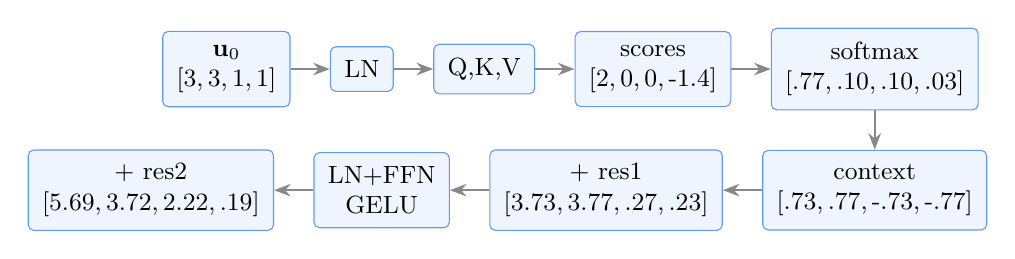
\begin{tikzpicture}[node distance=3.5mm and 5mm, font=\scriptsize]
\node[blkA] (x) {$\mathbf{u}_0$\\$[3,3,1,1]$};
\node[blkA, right=of x] (ln1) {LN};
\node[blkA, right=of ln1] (qkv) {Q,K,V};
\node[blkA, right=of qkv] (sc) {scores\\$[2,0,0,\text{-}1.4]$};
\node[blkA, right=of sc] (sm) {softmax\\$[.77,.10,.10,.03]$};
\node[blkA, below=5mm of sm] (ctx) {context\\$[.73,.77,\text{-}.73,\text{-}.77]$};
\node[blkA, left=of ctx] (r1) {$+$ res1\\$[3.73,3.77,.27,.23]$};
\node[blkA, left=of r1] (ffn) {LN+FFN\\GELU};
\node[blkA, left=of ffn] (r2) {$+$ res2\\$[5.69,3.72,2.22,.19]$};
\draw[ar](x)--(ln1);\draw[ar](ln1)--(qkv);\draw[ar](qkv)--(sc);\draw[ar](sc)--(sm);
\draw[ar](sm)--(ctx);\draw[ar](ctx)--(r1);\draw[ar](r1)--(ffn);\draw[ar](ffn)--(r2);
\end{tikzpicture}
\caption{Một lớp encoder cho token \code{[CLS]} bằng số (bản thu nhỏ $d{=}4$).}
\end{figure}

% ---------------------------------------------------------------
\subsection{Bước 3 --- lặp các lớp $\to$ head $\to$ logit $\to$ xác suất}
\label{sec:trace-head}
Model thật lặp khối trên 4 lần (baseline) / 6 lần (SE2); mỗi lần token
\code{[CLS]} hút thêm ngữ cảnh. Ở bản thu nhỏ ta coi $\mathbf{u}_0''$ là vector
\code{[CLS]} cuối, rồi đưa qua \textbf{classifier head} (LN $\to$ Linear).
LN$(\mathbf{u}_0'')$: $\mu=2.955$, $\sigma=2.015$ $\Rightarrow
\hat{\mathbf{h}}=[1.355,\,0.381,\,\text{-}0.363,\,\text{-}1.373]$.
Với trọng số head minh hoạ $w=[1,1,1,1],\ b=-0.5$:
\[
z=w\cdot\hat{\mathbf{h}}+b=(1.355{+}0.381{-}0.363{-}1.373)-0.5=0-0.5=\boxed{-0.5}
\quad(\text{logit}).
\]
\textbf{Xác suất FAIL}:
\[
p=\sigma(z)=\frac{1}{1+e^{-z}}=\frac{1}{1+e^{0.5}}=\frac{1}{2.649}=\boxed{0.378}.
\]
Đây chính là số $p$ ta đem đi \emph{xếp hạng} và tính APFD ở \S\ref{sec:apfd-example}.

% ---------------------------------------------------------------
\subsection{Bước 3' --- SE2RoadNet khác ở đâu: bias arclength trong attention}
\label{sec:trace-se2}
SE2RoadNet dùng \emph{đúng} các bước (b)--(h) trên, chỉ chèn thêm một
\textbf{bias} vào điểm attention ở bước (c), sinh từ \emph{hiệu độ dài cung}
$s_i-s_j$ (bất biến) --- \emph{thay cho} positional embedding tuyệt đối của
baseline. Gọi $s_{\text{norm}}$ của 3 điểm là $[0.2,0.5,0.8]$ và \code{[CLS]}
gán $s=0$, nên $s_{\text{full}}=[0,\,0.2,\,0.5,\,0.8]$.

\paragraph{(i) Ma trận hiệu arclength (hàng \code{[CLS]}).}
$\Delta s_{0j}=s_0-s_j=[\,0,\ -0.2,\ -0.5,\ -0.8\,]$.

\paragraph{(ii) Random Fourier features.} Với tần số cố định minh hoạ
$\boldsymbol\omega=[1.0,\,3.0]$ (thật: 32 tần số), một phần tử $\Delta s=-0.8$:
\[
\mathrm{feat}=\sin(\Delta s\cdot\boldsymbol\omega)=\sin([-0.8,\,-2.4])
=[\,-0.717,\ -0.675\,].
\]
Một MLP nhỏ $(32{\to}64{\to}\text{nhead})$ \emph{học} biến vector RFF này thành
\emph{một số bias cho mỗi head}. Trong bản thu nhỏ, hiệu ứng ròng của MLP đó xấp
xỉ ``phạt theo khoảng cách cung'': $b(\Delta s)\approx-2\,|\Delta s|$, cho hàng
\code{[CLS]}:
\[
\mathbf{b}=[\,0,\ -0.4,\ -1.0,\ -1.6\,].
\]

\paragraph{(iii) Điểm attention CÓ bias, rồi softmax.} Cộng $\mathbf{b}$ vào điểm
số thô $[2,0,0,-1.414]$ \emph{trước} softmax:
\[
s+b=[\,2.0,\ -0.4,\ -1.0,\ -3.014\,]\ \xrightarrow{\text{softmax}}\
\mathbf{a}^{\text{SE2}}=[\,0.872,\ 0.079,\ 0.043,\ 0.006\,].
\]
So với baseline $[0.767,0.104,0.104,0.025]$: bias theo arclength \emph{dồn} chú ý
vào token gần (theo độ dài cung) và \emph{ép} token xa (token 3, $s{=}0.8$) gần
như bằng 0 --- tất cả \emph{không} cần biết vị trí tuyệt đối, nên \textbf{bất
biến quay} (đã chứng minh ở \S\ref{sec:methodB}). Từ đây context/residual/FFN/
head chạy y hệt \S\ref{sec:trace-enc}--\ref{sec:trace-head} và cho một logit
riêng của SE2.

% ---------------------------------------------------------------
\subsection{Bước 4 --- hàm mất mát bằng số (Focal loss)}
\label{sec:trace-loss}
Giả sử ví dụ trên có \textbf{nhãn thật $y=1$ (FAIL)} và $p=0.378$. Tỉ lệ mất cân
bằng cho $\text{pos\_weight}=n_{\text{neg}}/n_{\text{pos}}=2.0$ (toy). Đi qua
đúng công thức \code{FocalLoss}:
\begin{align*}
\text{BCE}&=-\big[y\ln p+(1{-}y)\ln(1{-}p)\big]=-\ln(0.378)=0.974,\\
\text{trọng số lớp (}y{=}1\text{)}&=\text{pos\_weight}=2.0\ \Rightarrow\
\text{BCE}_w=2.0\times0.974=1.948,\\
p_t\ (\text{độ ``đúng''})&=p=0.378\quad(\text{vì }y{=}1),\\
\text{hệ số focal}&=(1-p_t)^\gamma=(0.622)^{2.5}=0.306\quad(\gamma{=}2.5\ \text{của baseline}),\\
\boxed{\text{loss}}&=\text{focal}\times\text{BCE}_w=0.306\times1.948=\boxed{0.596}.
\end{align*}

\paragraph{Focal ``tắt'' ví dụ dễ --- xem bằng số.} Lấy ví dụ B: PASS ($y{=}0$),
model đoán đúng tự tin $p=0.2$ (nên $p_t=1{-}p=0.8$):
\[
\text{BCE}=-\ln(0.8)=0.223,\quad
\text{focal}=(1-0.8)^{2.5}=0.2^{2.5}=0.0179,\quad
\text{loss}_B=0.0179\times0.223=\mathbf{0.004}.
\]
Ví dụ khó/sai (0.596) \emph{lấn át} ví dụ dễ đúng (0.004) gấp $\sim$150 lần ---
đó là mục đích của focal: dồn gradient vào biên PASS/FAIL. Mất mát của batch là
\emph{trung bình}:
\[
\mathcal{L}=\frac{0.596+0.004}{2}=\mathbf{0.300}.
\]
Nếu dùng $\gamma{=}0$ (BCE có trọng số thuần), hệ số focal $=1$ và loss ví dụ A là
$1.948$ --- tức focal đã \emph{hạ} nó xuống $0.596$. $\gamma$ càng lớn càng gắt;
baseline chọn $2.5$, SE2 (theo sweep) chọn $\gamma{=}1$ (hạ nhẹ hơn, giữ nhiều
tín hiệu cho lớp FAIL thiểu số --- xem \S\ref{sec:gammaB}).

% ---------------------------------------------------------------
\subsection{Bước 5 --- lan truyền ngược, cập nhật, và SWA}
\label{sec:trace-backward}
\begin{description}[leftmargin=0em,style=nextline]
\item[Backward] Từ $\mathcal{L}=0.300$, autograd tính $\partial\mathcal{L}/
\partial\theta$ cho \emph{mọi} tham số $\theta$ (các $W_{\text{in}},W_Q,W_K,W_V,
W_1,W_2$, head, \code{[CLS]}, pos-embedding\dots). Trực giác: vì ví dụ A (FAIL) bị
đoán $p{=}0.378$ quá thấp, gradient sẽ \emph{đẩy} các trọng số để lần sau logit
của nó cao hơn.
\item[Clip \& step] Chuẩn gradient bị cắt về $\le 1.0$ (\code{clip\_grad\_norm}),
rồi AdamW bước: $\theta\leftarrow\theta-\text{lr}\cdot\widetilde{g}$ với
$\text{lr}=5{\times}10^{-4}$ (đã nhân hệ số warmup/cosine của epoch đó).
\item[SWA] Ở $\sim$25 epoch cuối, thay vì lấy trọng số của \emph{một} epoch, ta
\emph{trung bình} chúng. Ví dụ một trọng số qua 2 snapshot $0.30$ và $0.40$:
\[
\bar\theta\ \xleftarrow{\ \text{snap 1}\ }0.30,\qquad
\bar\theta\ \xleftarrow{\ \text{snap 2}\ }(1-\tfrac12)0.30+\tfrac12(0.40)=0.35.
\]
Trung bình này nằm ở ``đáy phẳng'' $\Rightarrow$ tổng quát tốt hơn (cú nhảy APFD
lớn nhất của baseline: $0.7899\!\to\!0.8042$).
\end{description}

\paragraph{Toàn cảnh một vòng.}
\begin{center}\small
\code{đặc trưng} $\to$ \code{proj} $\to$ [\,LN$\to$attn$\to$softmax$\to$context$\to$res
$\to$LN$\to$FFN$\to$res\,]$\times L$ $\to$ \code{[CLS]} $\to$ \code{head} $\to$
$z\!=\!-0.5$ $\to$ $p\!=\!0.378$ $\to$ \code{FocalLoss}$=0.596$ $\to$ backward
$\to$ AdamW $\to$ (25 ep cuối) SWA.
\end{center}
Lặp vòng này 75--80 epoch trên hàng nghìn con đường là ra model cuối; đổi
\emph{bộ đặc trưng} + \emph{cách nhét vị trí} chính là toàn bộ khác biệt giữa hai
method.

% =====================================================================
\section{Tóm tắt một trang}
\label{sec:tldr}
\begin{itemize}[leftmargin=1.4em]
\item \textbf{Bài toán}: từ hình học con đường (dãy điểm 2D) đoán xác suất FAIL,
xếp hạng để lỗi lộ sớm; đo bằng \textbf{APFD}.
\item \textbf{Chung}: JSON $\to$ đặc trưng chuỗi $\to$ chuẩn hoá $\to$ Transformer
có \code{[CLS]} $\to$ logit $\to$ $\sigma$ $\to$ sắp xếp $\to$ APFD; huấn luyện
bằng Focal loss + \code{pos\_weight} + WeightedSampler + AdamW/cosine + AMP +
clip + \textbf{SWA}.
\item \chA{Method A (exp00)}: 10 kênh \emph{có heading tuyệt đối}, positional
\emph{tuyệt đối}, $d{=}128$/4 lớp, $\gamma{=}2.5$. Mạnh, đơn giản, nhưng
\emph{không} bất biến quay $\Rightarrow$ APFD tụt khi bản đồ xoay. Số chốt:
\textbf{APFD $0.8066\pm0.0124$}.
\item \chB{Method B (exp02 + exp02b, $\gamma{=}1$)}: 7 kênh \emph{nội tại},
attention dùng \emph{hiệu arclength} thay vị trí tuyệt đối, $d{=}192$/6 lớp.
\textbf{Bất biến SE(2) exact} ($\Delta_{\text{quay}}=0.0000$). Cùng kiến trúc
exp02, chỉ đổi focal $\gamma:1.5\!\to\!1$ theo bản quét \fileBb{}.
\item \textbf{Khác biệt cốt lõi chỉ ở 2 chỗ}: (i) bộ đặc trưng 10-vs-7 kênh,
(ii) cách nhét vị trí vào attention (tuyệt đối vs hiệu arclength). Mọi thứ khác
là chung.
\end{itemize}

\vspace{3mm}\hrule\vspace{2mm}
\noindent{\scriptsize Nguồn: \fileA{}, \fileB{}, \fileBb{} trong \code{exps/}.
Số APFD/tham số trích từ \code{exps/tracker.md}. Ô APFD cho SE2 $\gamma{=}1$ để
trống có chủ đích --- chạy \fileBb{} với \code{SDC\_GAMMAS="1.0"} để điền chính
xác.}

\end{document}
